\subsection{使用器具}
	ダイオードの特性実験の使用機材を以下の\wtab{diode_apparatus}に示す。

	\begin{table}[hbt]
		\centering
		\caption{使用器具}
		\begin{tabular}{|c||c|c|c|} \hline
				使用器具名 & 製造元 & 型番 & 製造番号(管理番号)\\ \hline
				電流計(ミリアンペア計) & YOKOGAWA & E-CLASS 1.0 & 48-2 \\ \hline
				電圧計 & YOKOGAWA & E-CLASS 1.0 & 278-20 \\ \hline
				電源装置 & YOKOGAWA & PA1811 & L69-000668 \\ \hline
		\end{tabular}
		\label{tab:diode_apparatus}
	\end{table}

% % % % % % % % % % % % % % % % % % % % % % % % % % % % % % % % % % % % % % % % % % % % % % % % % % % % % % 
\subsection{順バイアス}
\subsubsection{実験方法}
  順バイアスのダイオードの特性計測に用いた回路を\wfig{diode1_circuit} に示す。

  \begin{figure}[!h]
    \centering
    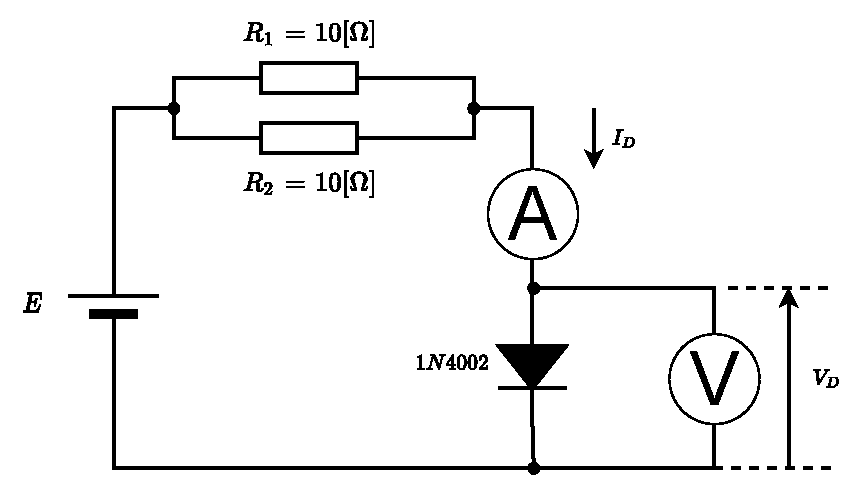
\includegraphics[width=10cm]{./pdfs/diode1.pdf}
    \caption{順バイアスのダイオードの回路図}
    \label{fig:diode1_circuit}
  \end{figure}

  この実験では直流電源Eの電圧を0.0~0.8 V まで0.1 V ずつ増加させた。
  そのときの電圧$V_D$,電流$I_D$を計測した。
  また,必要に応じて計測点を増やした。

\subsubsection{結果}
  計測して得られたデータを\wtab{diode1_result} に示す。
  また,\wtab{diode1_result} から作成したグラフを\wfig{forward_bias_ID-VD} に示す。
  このグラフから,順バイアスのときダイオードにかかる電圧が0.6 V 以上の場合,電流を通すことが分かる。
  また,0.6 V 以下の場合ほとんど電流を通さないことも分かる。
  約0.7 V から通す電流が著しく増加していることが分かる。

  \begin{table}[hbt]
    \centering
    \caption{順バイアスのダイオード特性の測定結果}
    \begin{tabular}{|c|c|} \hline
        電圧 & 電流 \\
        $V_D$ [V] & $I_D$ [mA] \\ \hline
        0.000 & 0.0 \\ \hline
        0.100 & 0.0 \\ \hline
        0.200 & 0.0 \\ \hline
        0.300 & 0.0 \\ \hline
        0.400 & 0.0 \\ \hline
        0.500 & 0.0 \\ \hline
        0.600 & 0.5 \\ \hline
        0.648 & 5.0 \\ \hline
        0.678 & 10.0 \\ \hline
        0.700 & 17.5 \\ \hline
        0.722 & 30.0 \\ \hline
        0.746 & 50.0 \\ \hline
        0.760 & 75.0 \\ \hline
        0.770 & 100.0 \\ \hline
        0.788 & 150.0 \\ \hline
        0.800 & 182.5 \\ \hline
    \end{tabular}
    \label{tab:diode1_result}
  \end{table}

  \begin{figure}[!h]
    \centering
    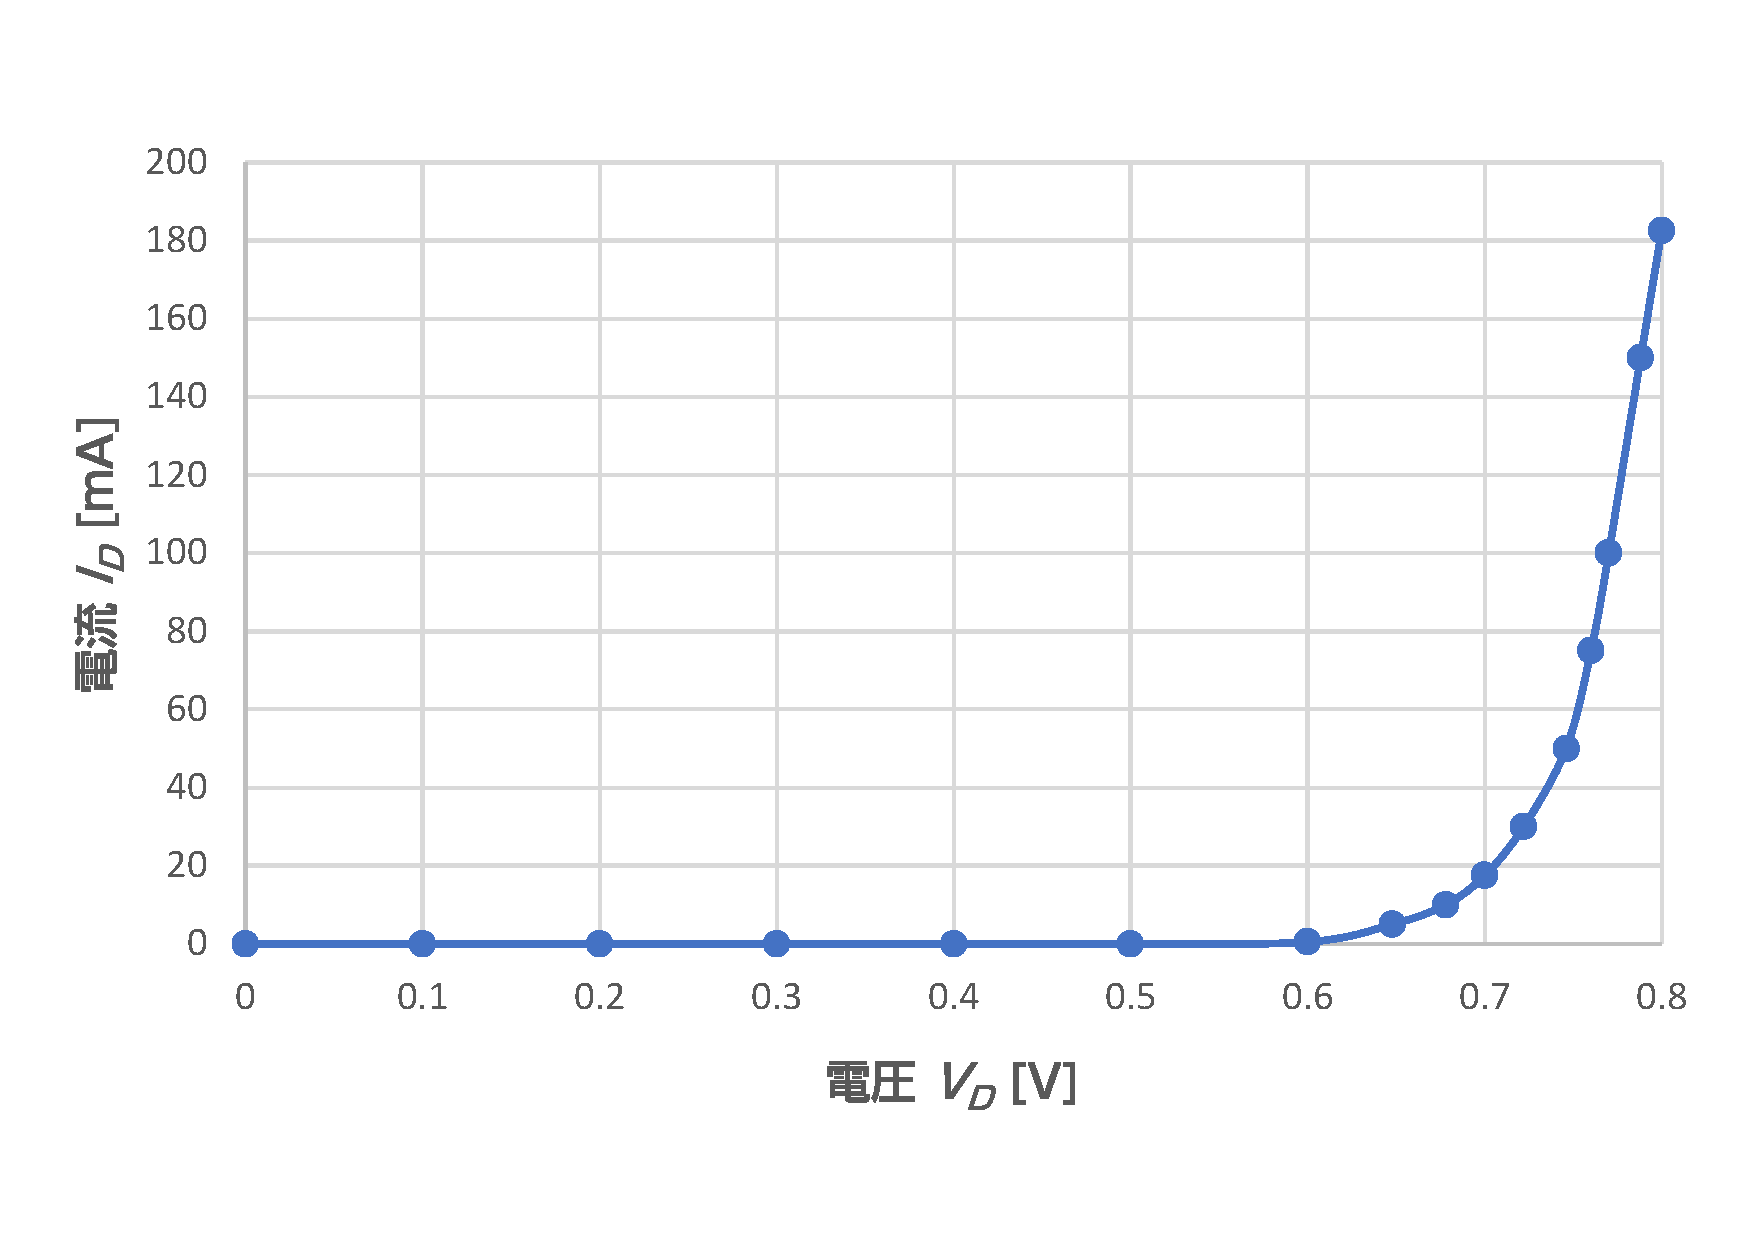
\includegraphics[width=13cm]{./figs/G-forward_bias_ID-VD.pdf}
    \caption{順バイアスのダイオードの電圧電流特性}
    \label{fig:forward_bias_ID-VD}
  \end{figure}

\newpage%%%%%
\subsubsection{考察}
  直流電圧電流特性グラフを説明せよ。\\

  \begin{figure}[!h]
    \centering
    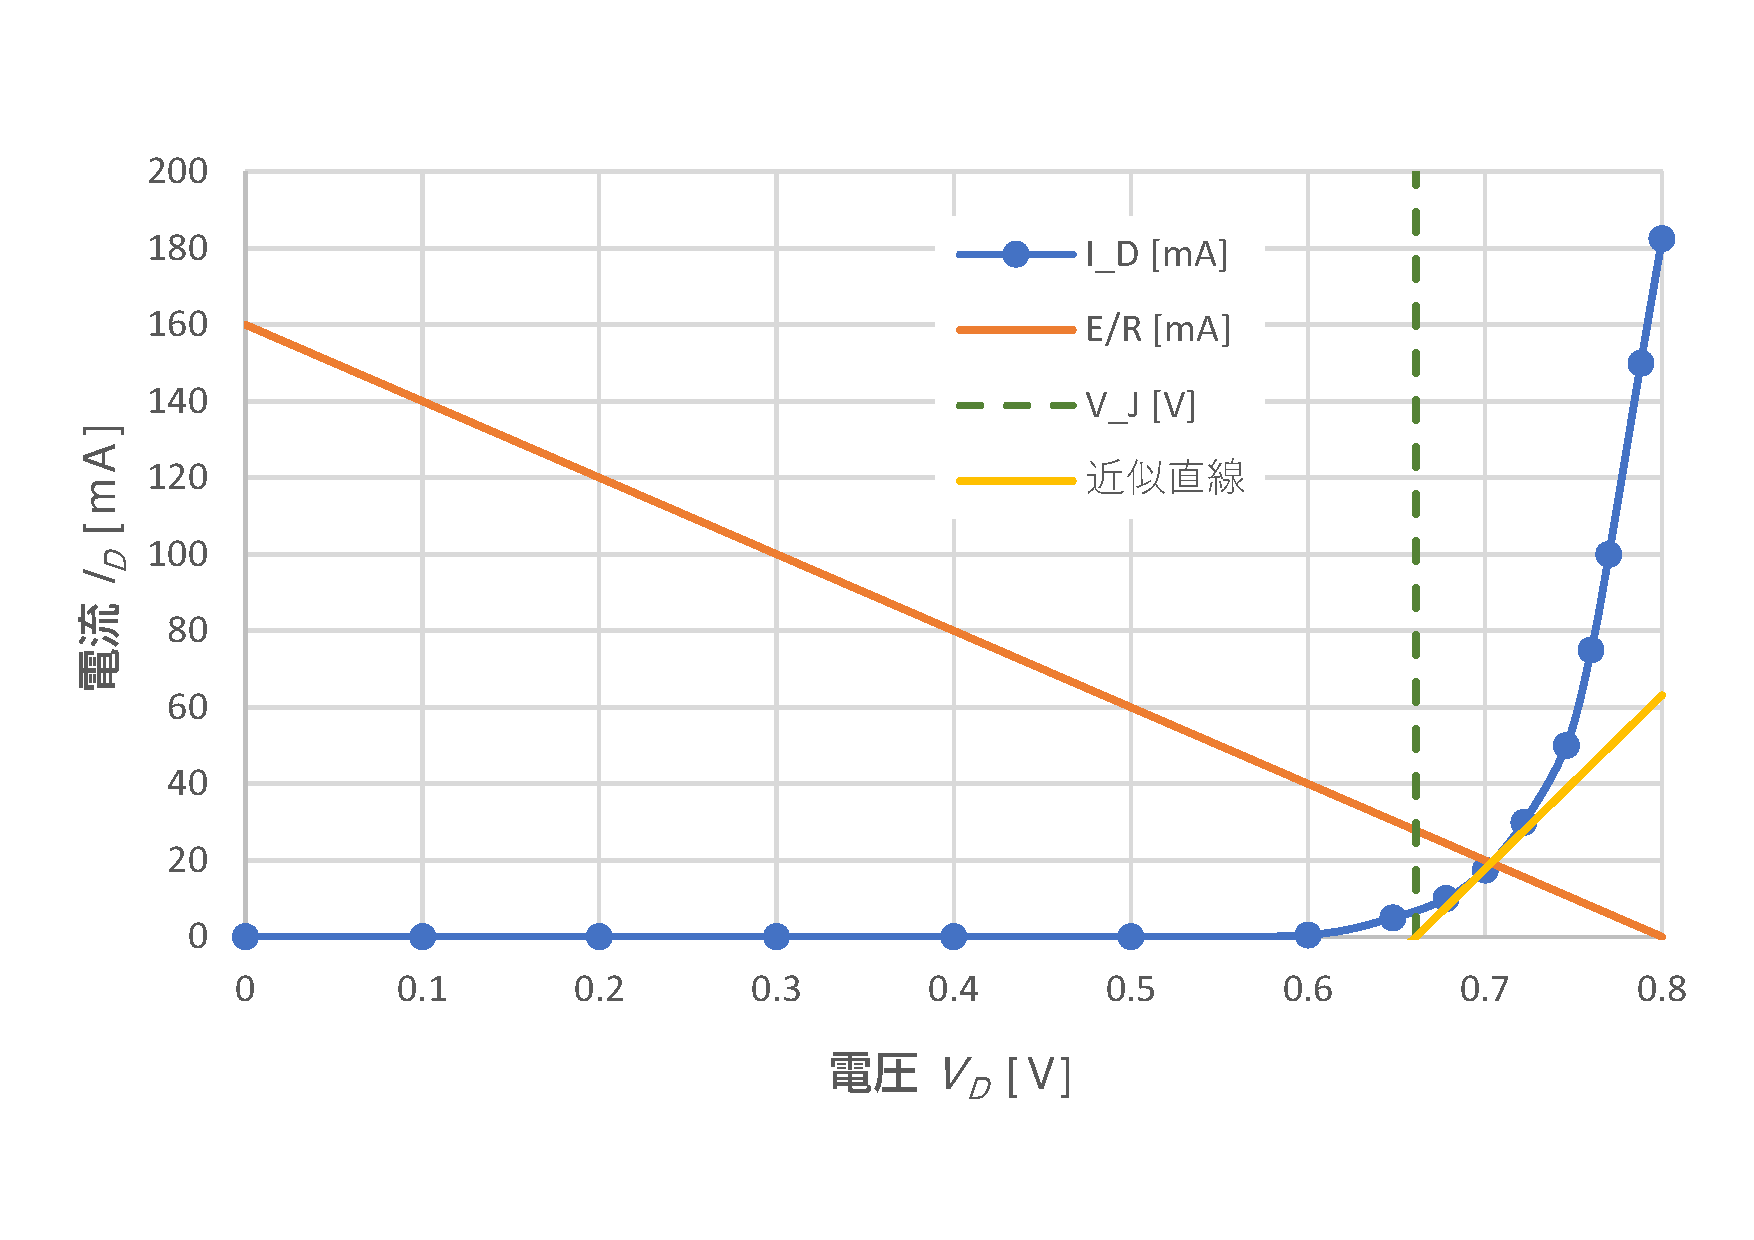
\includegraphics[width=13cm]{./figs/G-forward_discussion.pdf}
    \caption{順バイアス電流と負荷線と立ち上がり電圧}
    \label{fig:forward_discussion}
  \end{figure}
  
  \begin{table}[hbt]
    \centering
    \caption{tab:順バイアスの測定結果と負荷線と誤差}
    \begin{tabular}{|c|c|c|c|}
    \hline
    電圧 & 電流 & 電流 & 電流(誤差) \\
    $V_D$ [V] & $I_D$ [mA] & $E/R$ [mA] & $|I_D-E/R|$ [mA] \\ \hline
    0            & 0             & 160          & 160                 \\ \hline
    0.1          & 0             & 140          & 140                 \\ \hline
    0.2          & 0             & 120          & 120                 \\ \hline
    0.3          & 0             & 100          & 100                 \\ \hline
    0.4          & 0             & 80           & 80                  \\ \hline
    0.5          & 0             & 60           & 60                  \\ \hline
    0.6          & 0.5           & 40           & 39.5                \\ \hline
    0.648        & 5             & 30.4         & 25.4                \\ \hline
    0.678        & 10            & 24.4         & 14.4                \\ \hline
    0.7          & 17.5          & 20           & 2.5                 \\ \hline
    0.722        & 30            & 15.6         & 14.4                \\ \hline
    0.746        & 50            & 10.8         & 39.2                \\ \hline
    0.76         & 75            & 8            & 67                  \\ \hline
    0.77         & 100           & 6            & 94                  \\ \hline
    0.788        & 150           & 2.4          & 147.6               \\ \hline
    0.8          & 182.5         & 0            & 182.5               \\ \hline
    \end{tabular}
    \label{tab:diode1_}
  \end{table}

  \wfig{forward_discussion} は\wfig{forward_bias_ID-VD} に負荷線,接線の近似直線,立ち上がり電圧を追記したものだ。
  負荷線は$\frac{V_R}{R}$で計算した。
  $V_R$は抵抗にかかっている電圧であり,分圧則\cite{tyosho:denkiKiso1}より$V_R = E - V_D$($E=0.8\mathrm{[V]}$)と計算した。
  $R$は$R_1$と$R_2$の合成抵抗と考え,\weq{resistance_calc} のように計算した。
  よって,合成抵抗$R=5[\Omega]$ である。
  \begin{align}
    R &= \frac{R_1*R_2}{R_1 + R_2} \nonumber \\
    &= \frac{10*10}{10 + 10} \nonumber \\
    &= 5 \label{eq:resistance_calc}
  \end{align}
  接線の近似直線は以下の手順で求めた。
  \begin{enumerate}
    \item $I_D$と$E/R$の誤差を計算する。
    \item $V_D = 0.7 \mathrm{[V]}$で最も誤差が小さくなっているので,$V_D = 0.7 \mathrm{[V]}$に近い前後2点から傾きを計算する。
        \begin{align}
          \begin{cases}
            dV_D &= 0.722 - 0.678 \nonumber \\
            &= 0.044 \mathrm{[V]} \nonumber \\
            dI_D &= 30 - 10 \nonumber \\
            &= 20 \mathrm{[mA]} \nonumber \\
          \end{cases} \nonumber \\
          \frac{dI_D}{dV_D} &= \frac{20}{0.044} \nonumber \\
          &\approx 454.5 \label{eq:approxLine_calc}
        \end{align}
    \item 以下の式に$V_D = 0.7 \mathrm{[V]}$のときの値を代入し,$V_J$(x切片)を計算する。
        \begin{align}
          I_D &= \frac{dI_D}{dV_D} (V_D - V_J) \nonumber \\
          \begin{cases}
            \frac{dI_D}{dV_D} &= 454.5 \nonumber \\
            V_D &= 0.700 \nonumber \\
            I_D &= 17.5 \nonumber \\
          \end{cases} \nonumber \\
          17.5 &= 454.5(0.700 - V_J) \nonumber \\
          V_J &\approx 0.661 \mathrm{[V]} \nonumber
        \end{align}
    \item よって下式が接線の近似直線の式である。
        \begin{equation}
          I = 454.5 (V - 0.661) \mathrm{[mA]} \label{eq:approxLine}
        \end{equation}
  \end{enumerate}
  立ち上がり電圧は接線の近似直線と$I = 0 \mathrm{[mA]}$の交点である。
  $I = 0 \mathrm{[mA]}$を\weq{approxLine} に代入すると,V = 0.661 [V] である。
  よって,立ち上がり電圧は 0.661 V である。

  微分抵抗$r_d$は\weq{approxLine_calc} の$\frac{dI_D}{dV_D}$の分母と分子を入れ替えることで計算できる。
  よって$r_d$は以下のようにして求めれられる。
  \begin{equation}
    r_d = \frac{dI_D}{dV_D} = \frac{0.044}{20*10^{-3}} = 2.2 \mathrm{[\Omega]} \nonumber
  \end{equation}
  
  \wfig{risou1} は$r_d$,$V_J$,理想ダイオードで構成された等価回路である。
  $r_d$はダイオードの抵抗成分を示し,$V_J$はダイオードの内部で発生する電界から生まれる電圧降下を示す。
  理想ダイオードはダイオードの整流作用を示す。
  \begin{figure}[!h]
    \centering
    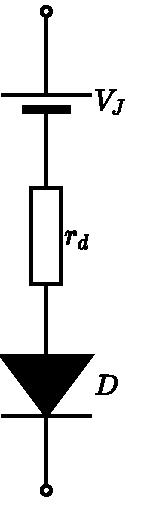
\includegraphics[width=2cm]{./pdfs/risou1.pdf}
    \caption{順バイアスのダイオードの等価回路}
    \label{fig:risou1}
  \end{figure}

% % % % % % % % % % % % % % % % % % % % % % % % % % % % % % % % % % % % % % % % % % % % % % % % % % % % % % 
\subsection{逆バイアス}
\subsubsection{実験方法}
  逆バイアスのダイオードの特性計測に用いた回路を\wfig{diode2_circuit} に示す。

  \begin{figure}[!h]
    \centering
    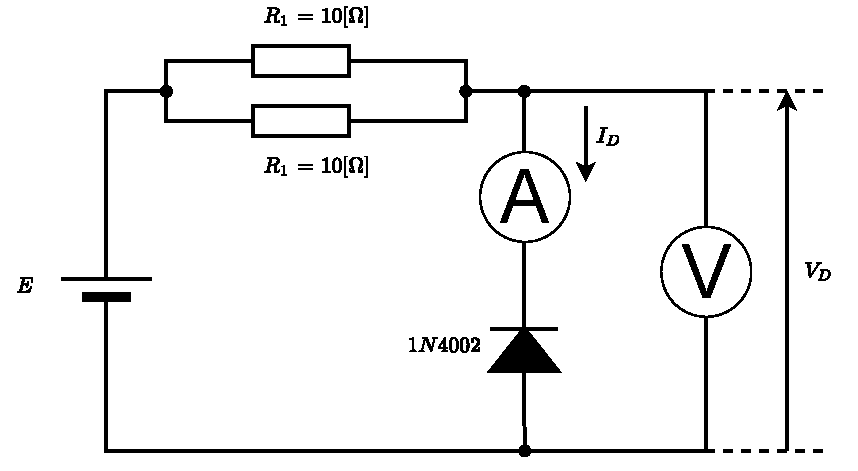
\includegraphics[width=10cm]{./pdfs/diode2.pdf}
    \caption{逆バイアスのダイオードの回路図}
    \label{fig:diode2_circuit}
  \end{figure}

  この実験では直流電源Eの電圧を0~8 V まで1 V ずつ増加させた。
  そのときの電圧$V_D$,電流$I_D$を計測した。

\subsubsection{結果}
  計測して得られたデータを\wtab{diode1_result} に示す。
  また,\wtab{diode1_result} から作成したグラフを\wfig{reverse_bias_ID-VD} に示す。
  このグラフから,逆バイアスのときダイオードにかかる電圧が8 V になっても,ダイオードは電流を通さないことが分かる。
  また,\wfig{forward_bias_ID-VD} と比べて,非常に高い電圧になっても電流を通さないことも分かる。
  このことから,ダイオードの整流作用\cite{tyosho:densiKairo} を確認できる。

  \begin{table}[hbt]
    \centering
    \caption{逆バイアスのダイオード特性の測定結果}
    \begin{tabular}{|c|c|} \hline
        電圧 & 電流 \\
        $V_D$ [V] & $I_D$ [mA] \\ \hline
        0 & 0 \\ \hline
        1 & 0 \\ \hline
        2 & 0 \\ \hline
        3 & 0 \\ \hline
        4 & 0 \\ \hline
        5 & 0 \\ \hline
        6 & 0 \\ \hline
        7 & 0 \\ \hline
        8 & 0 \\ \hline
    \end{tabular}
    \label{tab:diode2_result}
  \end{table}

  \begin{figure}[!h]
    \centering
    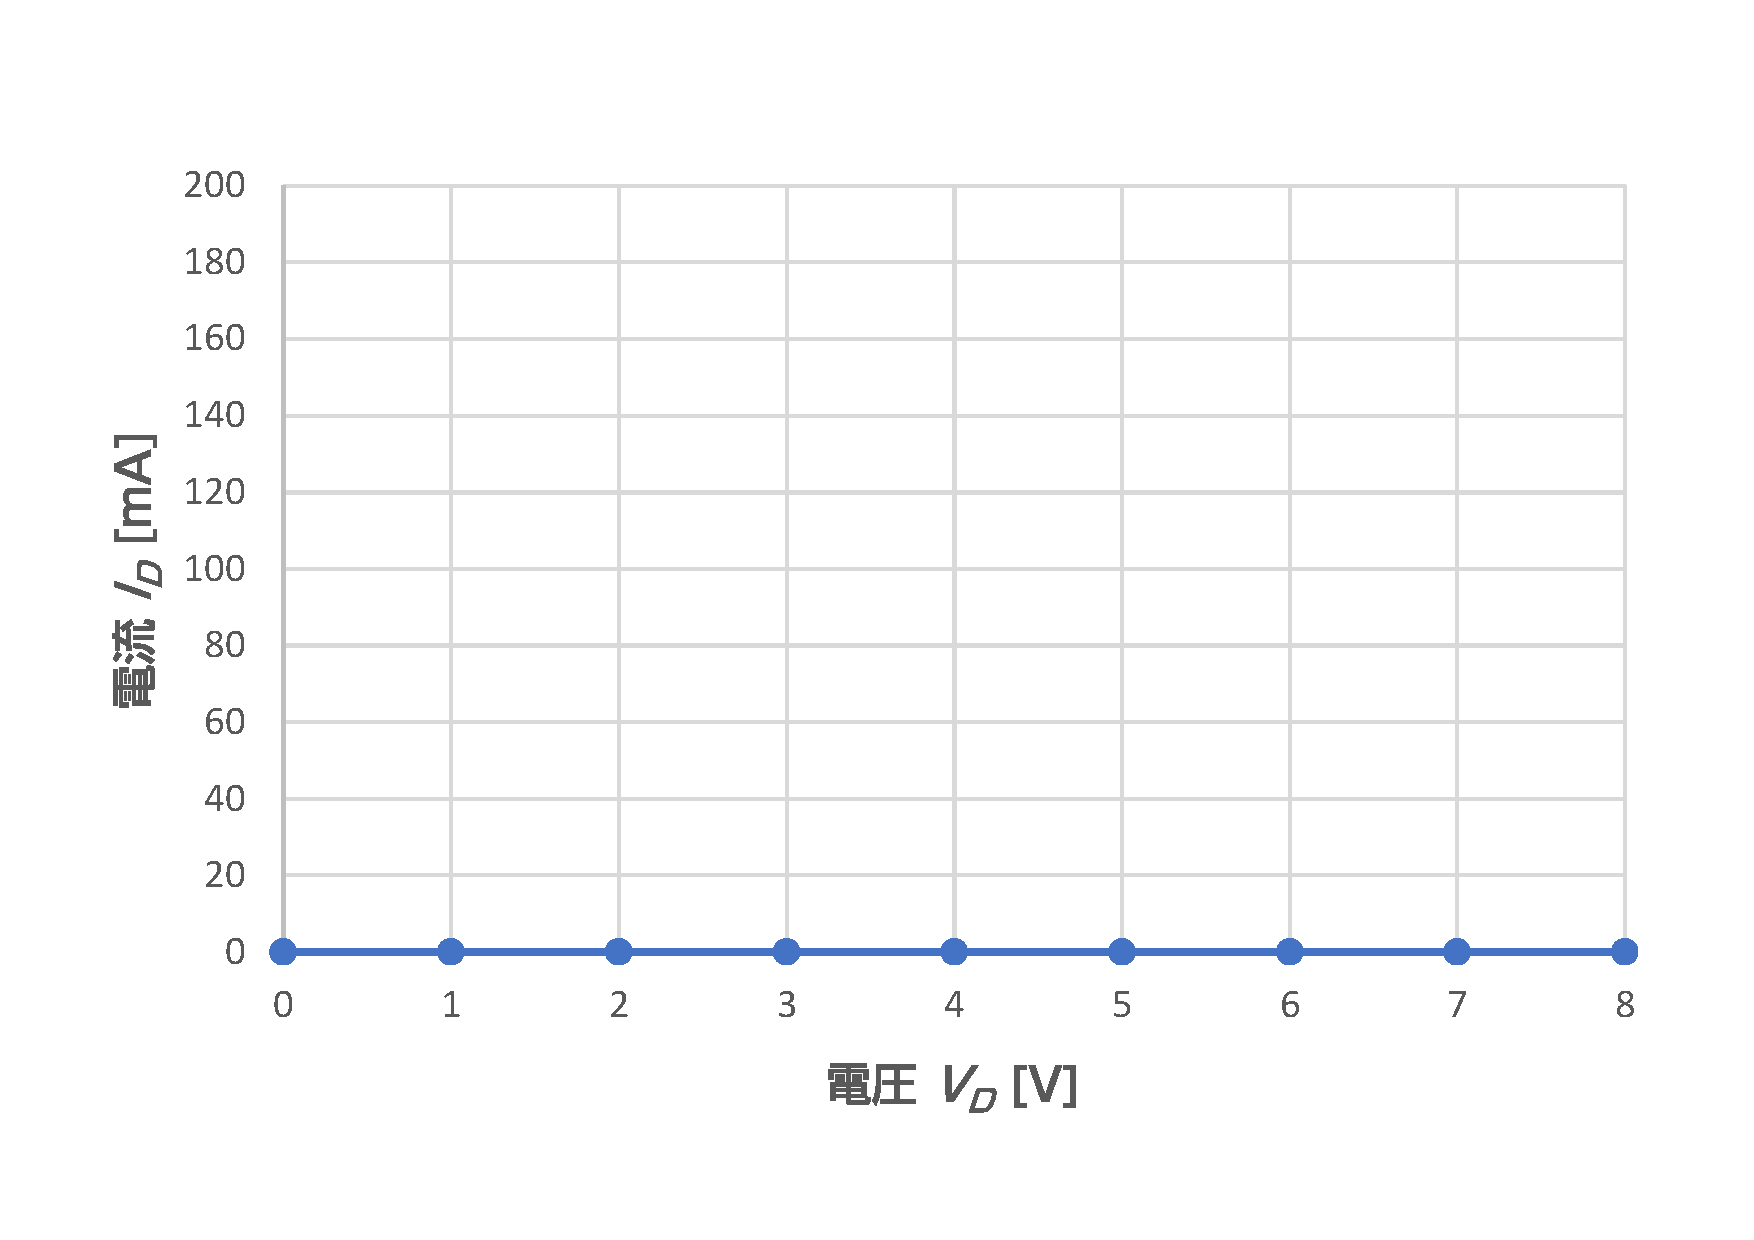
\includegraphics[width=8.2cm]{./figs/G-reverse_bias_ID-VD}
    \caption{逆バイアスのダイオードの電圧電流特性}
    \label{fig:reverse_bias_ID-VD}
  \end{figure}

\subsubsection{考察}
  実験で用いたダイオードのデータシートから逆方向電流の値を調べよ。
  また,逆バイアスの場合でもわずかに電流が流れる理由を図を用いて説明せよ。

  1N4001のデータシート\cite{web:1N4001} によると,ダイオード1N4002は逆バイアス時に 5 uA のドリフト電流を流す。
  ダイオードに逆バイアスをかけたとき,  n型p型ともに多数キャリアが再結合で減少する。
  また,同時に少数キャリアが移動する。
  このときの少数の電子の移動によりドリフト電流が流れる。
  \wfig{2} では多数キャリアに注目しているので,電子は移動せず電流は流れないように考えられる。
  しかし,p型半導体の少数キャリアの電子が移動するため,僅かに電流は流れてしまう。
